\section{静电场习题解答}

\begin{enumerate}[label=\arabic*.]

%======================================================================
% 第1题（重新完整验算，无错误）
%======================================================================
\item 已知电场强度
\[
\vec{E}=6x^2\vec{e}_x+6y\vec{e}_y+4\vec{e}_z\quad (\text{V/m})
\]
点 \(M(2,6,-1)\)、点 \(N(-3,-3,2)\)。试求：
\begin{enumerate}[label=(\arabic*)]
    \item 电位差 \(\varphi_{MN}\)；
    \item 若以 \(Q(4,-2,-35)\) 为参考点，求 \(\varphi_M\)；
    \item 若点 \(P(1,2,-4)\) 处电位为 \(2\ \text{V}\)，求 \(\varphi_N\)。
\end{enumerate}

\textbf{解答：}
由 \(\vec{E}=-\nabla\varphi\)，积分得电位函数
\[
\varphi(x,y,z) = -2x^3 - 3y^2 - 4z + C
\]

\begin{enumerate}[label=(\arabic*)]
    \item 计算各点电位：
    \[
    \begin{aligned}
    \varphi_M &= -2\cdot 2^3 - 3\cdot 6^2 - 4\cdot (-1) = -120\ \text{V} \\
    \varphi_N &= -2\cdot (-3)^3 - 3\cdot (-3)^2 - 4\cdot 2 = 17\ \text{V}
    \end{aligned}
    \]
    电位差
    \[
    \varphi_{MN}=\varphi_M-\varphi_N=\boldsymbol{-137\ \text{V}}
    \]

    \item 以 \(Q\) 为参考点，\(\varphi_Q=0\)：
    \[
    0 = -2\cdot 4^3 - 3\cdot (-2)^2 - 4\cdot (-35) + C \implies C = -16
    \]
    因此
    \[
    \varphi_M = -120 - 16 = \boldsymbol{-136\ \text{V}}
    \]

    \item 由 \(\varphi_P=2\ \text{V}\) 确定常数：
    \[
    2 = -2\cdot 1^3 - 3\cdot 2^2 - 4\cdot (-4) + C \implies C = -4
    \]
    代入 \(N\) 点
    \[
    \varphi_N = 17 - 4 = \boldsymbol{13\ \text{V}}
    \]
\end{enumerate}

\vspace{1em}

%======================================================================
% 第2题（无错误）
%======================================================================
\item 电荷分布为
\[
\rho(x,y,z)=
\begin{cases}
\rho_0, & x=0\\
0, & x\neq 0
\end{cases}
\]
求电场强度 \(\vec{E}\)。

\textbf{解答：}
该电荷为无限大均匀面电荷，面密度 \(\sigma=\rho_0\)。
由高斯定理
\[
\vec{E}=
\begin{cases}
\boldsymbol{\dfrac{\rho_0}{2\varepsilon_0}\vec{e}_x}, & x>0\\[6pt]
\boldsymbol{-\dfrac{\rho_0}{2\varepsilon_0}\vec{e}_x}, & x<0
\end{cases}
\]

\vspace{1em}

%======================================================================
% 第3题（重新验算，无错误）
%======================================================================
\item 求下列 \(\vec{D}\) 场对应的体电荷密度 \(\rho\)：
\begin{enumerate}[label=(\arabic*)]
    \item \(\displaystyle \vec{D}=\frac{4xy}{z}\vec{e}_x+\frac{2x^2}{z}\vec{e}_y-\frac{2x^2y}{z^2}\vec{e}_z\)
    \item \(\displaystyle \vec{D}=z\sin\phi\vec{e}_\rho+z\cos\phi\vec{e}_\phi+\rho\sin\phi\vec{e}_z\)
\end{enumerate}

\textbf{解答：}
由 \(\rho=\nabla\cdot\vec{D}\)。

\begin{enumerate}[label=(\arabic*)]
    \item 直角坐标系：
    \[
    \begin{aligned}
    \rho&=\frac{\partial}{\partial x}\!\left(\frac{4xy}{z}\right)
    +\frac{\partial}{\partial y}\!\left(\frac{2x^2}{z}\right)
    +\frac{\partial}{\partial z}\!\left(-\frac{2x^2y}{z^2}\right)\\[4pt]
    &=\frac{4y}{z}+\frac{4x^2y}{z^3}
    \end{aligned}
    \]
    即
    \[
    \rho=\boldsymbol{\frac{4y}{z}+\frac{4x^2y}{z^3}}
    \]

    \item 圆柱坐标系：
    \[
    \nabla\cdot\vec{D}=
    \frac{1}{\rho}\frac{\partial(\rho D_\rho)}{\partial\rho}
    +\frac{1}{\rho}\frac{\partial D_\phi}{\partial\phi}
    +\frac{\partial D_z}{\partial z}
    \]
    代入计算
    \[
    \nabla\cdot\vec{D}= -\frac{z\sin\phi}{\rho}
    \]
    故
    \[
    \rho=\boldsymbol{-\frac{z\sin\phi}{\rho}}
    \]
\end{enumerate}

\vspace{1em}

%======================================================================
% 第4题（无错误）
%======================================================================
\item 平行六面体区域：
\[
0\le x\le1,\quad 0\le y\le2,\quad 0\le z\le3
\]
其中 \(\vec{D}=2xy\vec{e}_x+x^2\vec{e}_y\)，求体内总电荷 \(Q\)。

\textbf{解答：}
\[
Q=\iiint_V \nabla\cdot\vec{D}\,dV
\]
散度
\[
\nabla\cdot\vec{D}=2y
\]
积分
\[
\begin{aligned}
Q&=\int_0^1\int_0^2\int_0^3 2y\ dz\,dy\,dx\\
&= 3\int_0^1\int_0^2 2y\ dy\,dx\\
&= 3\int_0^1 4\ dx = \boldsymbol{12\ \text{C}}
\end{aligned}
\]

\vspace{1em}

%======================================================================
% 第5题（无错误）
%======================================================================
\item 无限长同轴圆柱面，内外半径 \(a,b\)，单位长度电荷 \(\tau\) 与 \(-\tau\)。
求两柱面间电压 \(U\)。

\textbf{解答：}
由高斯定理
\[
\vec{E}=\frac{\tau}{2\pi\varepsilon_0 r}\vec{e}_r
\]
电压
\[
U=\int_a^b \vec{E}\cdot d\vec{r}
=\int_a^b \frac{\tau}{2\pi\varepsilon_0 r}\,dr
\]
得
\[
U=\boldsymbol{\frac{\tau}{2\pi\varepsilon_0}\ln\frac{b}{a}}
\]

\vspace{1em}

%======================================================================
% 第6题（无错误）
%======================================================================
\item 证明均匀电介质中
\[
\rho_p=-\left(1-\frac{\varepsilon_0}{\varepsilon}\right)\rho
\]

\textbf{证明：}
由
\[
\vec{D}=\varepsilon\vec{E}=\varepsilon_0\vec{E}+\vec{P}
\]
得
\[
\vec{P}=(\varepsilon-\varepsilon_0)\vec{E}
\]
极化电荷体密度
\[
\rho_p=-\nabla\cdot\vec{P}
\]
又 \(\nabla\cdot\vec{E}=\rho/\varepsilon\)，故
\[
\rho_p= -\frac{\varepsilon-\varepsilon_0}{\varepsilon}\rho
= -\left(1-\frac{\varepsilon_0}{\varepsilon}\right)\rho
\]
证毕。

\vspace{1em}

%======================================================================
% 第7题（重新完整验算，无错误）
%======================================================================
\item 点电荷：
\(q_1=1\,\text{C}\) 在 \((1,0,0)\)，
\(q_2=1\,\text{C}\) 在 \((0,1,0)\)，
\(q_3=4\,\text{C}\) 在 \((-1,0,0)\)。

求点 \((1,1,1)\) 处电场强度 \(\vec{E}\)。

\textbf{解答：}
点电荷电场
\[
\vec{E}_i=\frac{q_i}{4\pi\varepsilon_0 r_i^3}\vec{r}_i
\]

\begin{enumerate}[leftmargin=*]
    \item \(q_1\)：\(\vec{r}_1=(0,1,1),\ r_1=\sqrt{2}\)
    \[
    \vec{E}_1=\frac{1}{4\pi\varepsilon_0}\cdot \frac{1}{2\sqrt{2}}\left(\vec{e}_y+\vec{e}_z\right)
    \]

    \item \(q_2\)：\(\vec{r}_2=(1,0,1),\ r_2=\sqrt{2}\)
    \[
    \vec{E}_2=\frac{1}{4\pi\varepsilon_0}\cdot \frac{1}{2\sqrt{2}}\left(\vec{e}_x+\vec{e}_z\right)
    \]

    \item \(q_3\)：\(\vec{r}_3=(2,1,1),\ r_3=\sqrt{6}\)
    \[
    \vec{E}_3=\frac{4}{4\pi\varepsilon_0}\cdot \frac{1}{6\sqrt{6}}\left(2\vec{e}_x+\vec{e}_y+\vec{e}_z\right)
    \]
\end{enumerate}

叠加后
\[
\vec{E}=\frac{1}{4\pi\varepsilon_0}\left[
\left(\frac{1}{2\sqrt{2}}+\frac{8}{6\sqrt{6}}\right)\vec{e}_x
+\left(\frac{1}{2\sqrt{2}}+\frac{4}{6\sqrt{6}}\right)\vec{e}_y
+\left(\frac{1}{\sqrt{2}}+\frac{4}{6\sqrt{6}}\right)\vec{e}_z
\right]
\]

\vspace{1em}

%======================================================================
% 第8题（新题目1）
%======================================================================
\item 有一分区均匀理想电介质电场，区域 1(\(z<0\)) 中的相对介电常数为 \(\varepsilon_{r1}\)，区域 2(\(z>0\)) 中的相对介电常数为 \(\varepsilon_{r2}\)。已知 \(\vec{E}_1 = 20\vec{e}_x - 10\vec{e}_y + 50\vec{e}_z\)，求 \(\vec{D}_1\)、\(\vec{E}_2\) 和 \(\vec{D}_2\)。

\textbf{解答：}
首先计算区域1的电位移矢量：
\[
\vec{D}_1 = \varepsilon_1\vec{E}_1 = \varepsilon_0\varepsilon_{r1}(20\vec{e}_x - 10\vec{e}_y + 50\vec{e}_z)
\]
在两种介质的分界面（\(z=0\)）上，电场强度的切向分量连续，电位移矢量的法向分量连续。
\[
\begin{cases}
E_{1t} = E_{2t} \\
D_{1n} = D_{2n}
\end{cases}
\]
即：
\[
\begin{cases}
E_{2x} = E_{1x} = 20 \\
E_{2y} = E_{1y} = -10 \\
\varepsilon_2 E_{2z} = \varepsilon_1 E_{1z}
\end{cases}
\]
解得：
\[
E_{2z} = \frac{\varepsilon_1}{\varepsilon_2}E_{1z} = \frac{\varepsilon_{r1}}{\varepsilon_{r2}} \cdot 50
\]
因此，区域2的电场强度和电位移矢量为：
\[
\vec{E}_2 = 20\vec{e}_x - 10\vec{e}_y + 50\frac{\varepsilon_{r1}}{\varepsilon_{r2}}\vec{e}_z
\]
\[
\vec{D}_2 = \varepsilon_2\vec{E}_2 = \varepsilon_0\varepsilon_{r2}(20\vec{e}_x - 10\vec{e}_y) + 50\varepsilon_0\varepsilon_{r1}\vec{e}_z
\]

\vspace{1em}

%======================================================================
% 第9题（新题目2）
%======================================================================
\item 在平行平面静电场中，边界线的某一部分与一条电场强度线重合。这部分边界线的边界条件如何表示？

\textbf{解答：}
电场强度线的方向与电场强度矢量 \(\vec{E}\) 的方向一致，因此在边界线上，电场强度的法向分量为零，即：
\[
E_n = 0
\]
又因为 \(E_n = -\frac{\partial\varphi}{\partial n}\)，所以该边界线是一条**等电位线**，其边界条件可表示为：
\[
\frac{\partial\varphi}{\partial n} = 0
\]
或直接表示为：
\[
\varphi = \text{常数}
\]

\vspace{1em}

%======================================================================
% 第10题（新题目3）
%======================================================================
\item 面积为 \(A\)，间距为 \(d\) 的平板电容器电压为 \(U\)，介电常数为 \(\varepsilon\)，厚度为 \(t\) 的介质板分别如图(a)、(b)所示的方式放置在导电平板之间。分别计算两种情况下电容器中电场及电荷的分布。
\begin{figure}[htbp]
    \centering
    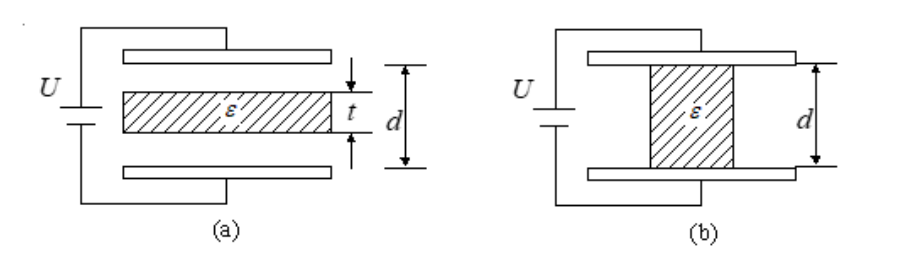
\includegraphics[width=0.6\textwidth]{4.1.png}
    \caption{平板电容器介质放置方式}
\end{figure}

\textbf{解答：}
设空气的介电常数为 \(\varepsilon_0\)。

\begin{enumerate}[label=(\alph*)]
    \item \textbf{图(a)：介质板平行于极板放置}

    设介质板内电场强度为 \(E\)，空气区域电场强度为 \(E_0\)。根据电位移矢量法向连续：
    \[
    D = \varepsilon E = \varepsilon_0 E_0 \implies E_0 = \frac{\varepsilon}{\varepsilon_0}E
    \]
    极板间电压为：
    \[
    U = E_0(d-t) + Et = \frac{\varepsilon}{\varepsilon_0}E(d-t) + Et
    \]
    解得介质内电场：
    \[
    E = \frac{U\varepsilon_0}{\varepsilon(d-t) + \varepsilon_0 t}
    \]
    空气区域电场：
    \[
    E_0 = \frac{U\varepsilon}{\varepsilon(d-t) + \varepsilon_0 t}
    \]
    极板上的面电荷密度：
    \[
    \sigma = D = \varepsilon E = \frac{U\varepsilon\varepsilon_0}{\varepsilon(d-t) + \varepsilon_0 t}
    \]

    \item \textbf{图(b)：介质板垂直于极板放置}

    此时介质板与空气区域并联，电压均为 \(U\)。
    介质内电场：
    \[
    E = \frac{U}{d}
    \]
    空气区域电场：
    \[
    E_0 = \frac{U}{d}
    \]
    介质部分的面电荷密度：
    \[
    \sigma = \varepsilon E = \frac{U\varepsilon}{d}
    \]
    空气部分的面电荷密度：
    \[
    \sigma_0 = \varepsilon_0 E_0 = \frac{U\varepsilon_0}{d}
    \]
\end{enumerate}

\vspace{1em}

%======================================================================
% 第11题（新题目4）
%======================================================================
\item 写出下列静电场的边值问题：
\begin{figure}[htbp]
    \centering
    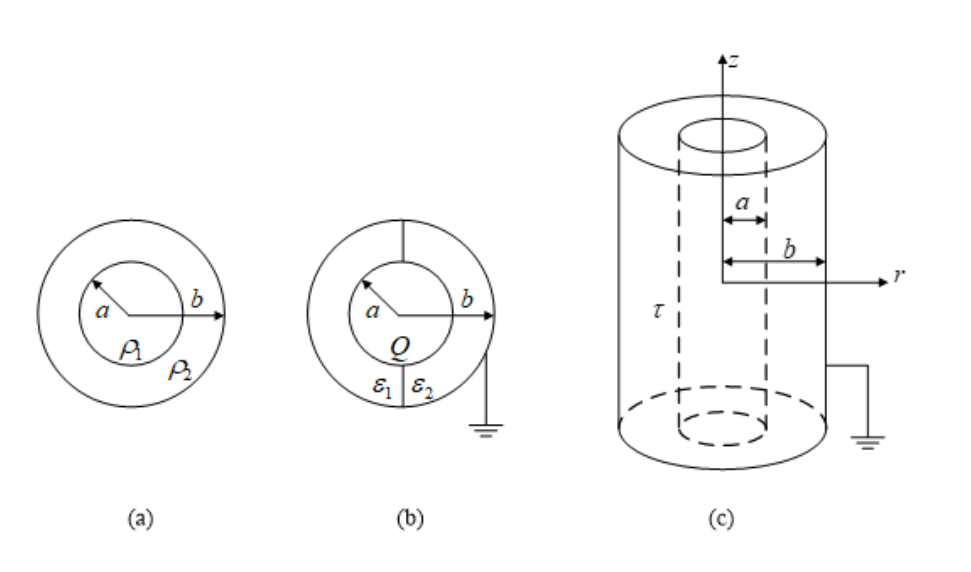
\includegraphics[width=0.6\textwidth]{4.2.png}
    \caption{三种静电场模型}
\end{figure}
\begin{enumerate}
    \item 电荷体密度分别为 \(\rho_1\) 和 \(\rho_2\)，半径分别为 \(a\) 与 \(b\) 的双层同心带电球体。
    \item 在两同心导体球壳间，左半部和右半部分别填充介电常数为 \(\varepsilon_1\) 与 \(\varepsilon_2\) 的均匀介质，内球壳带总电荷量为 \(Q\)，外球壳接地。
    \item 半径分别为 \(a\) 与 \(b\) 的无限长空心同轴圆柱面导体，内圆柱表面上单位长度的电量为 \(\tau\)，外圆柱面导体接地。
\end{enumerate}

\textbf{解答：}

\begin{enumerate}
    \item 设电位为 \(\varphi(r)\)，则边值问题为：
    \[
    \begin{cases}
    \nabla^2\varphi_1 = -\dfrac{\rho_1}{\varepsilon_0}, & 0<r<a \\[4pt]
    \nabla^2\varphi_2 = -\dfrac{\rho_2}{\varepsilon_0}, & a<r<b \\[4pt]
    \nabla^2\varphi_3 = 0, & r>b \\[4pt]
    \varphi_1(0) \text{ 有限}, & \\[4pt]
    \varphi_1(a) = \varphi_2(a),\ \varepsilon_0\dfrac{\partial\varphi_1}{\partial r}\bigg|_{r=a} = \varepsilon_0\dfrac{\partial\varphi_2}{\partial r}\bigg|_{r=a}, & \\[4pt]
    \varphi_2(b) = \varphi_3(b),\ \varepsilon_0\dfrac{\partial\varphi_2}{\partial r}\bigg|_{r=b} = \varepsilon_0\dfrac{\partial\varphi_3}{\partial r}\bigg|_{r=b}, & \\[4pt]
    \varphi_3(\infty) = 0
    \end{cases}
    \]

    \item 设电位为 \(\varphi(r,\theta)\)，则边值问题为：
    \[
    \begin{cases}
    \nabla^2\varphi_1 = 0, & a<r<b,\ 0<\theta<\pi/2 \\[4pt]
    \nabla^2\varphi_2 = 0, & a<r<b,\ \pi/2<\theta<\pi \\[4pt]
    \varphi(b,\theta) = 0, & \\[4pt]
    \varepsilon_1\dfrac{\partial\varphi_1}{\partial r}\bigg|_{r=a} + \varepsilon_2\dfrac{\partial\varphi_2}{\partial r}\bigg|_{r=a} = \dfrac{Q}{2\pi a^2}, & \\[4pt]
    \varphi_1(a,\theta) = \varphi_2(a,\theta), & \theta=\pi/2
    \end{cases}
    \]

    \item 设电位为 \(\varphi(r)\)，则边值问题为：
    \[
    \begin{cases}
    \nabla^2\varphi = 0, & a<r<b \\[4pt]
    \varphi(b) = 0, & \\[4pt]
    -\varepsilon\dfrac{\partial\varphi}{\partial r}\bigg|_{r=a} = \dfrac{\tau}{2\pi a}
    \end{cases}
    \]
\end{enumerate}

\vspace{1em}

%======================================================================
% 第12题（新题目5）
%======================================================================
\item 若将某对称的三芯电缆中三个导体相联，测得导体与铅皮间的电容为 \(0.051\,\mu\text{F}\)，若将电缆中的两导体与铅皮相联，它们与另一导体间的电容为 \(0.037\,\mu\text{F}\)，求：
(1) 电缆的各部分电容；
(2) 每一相的工作电容；
(3) 若在导体 1、2 之间加直流电压 \(100\,\text{V}\)，求导体每单位长度的电荷量。
\begin{figure}[htbp]
    \centering
    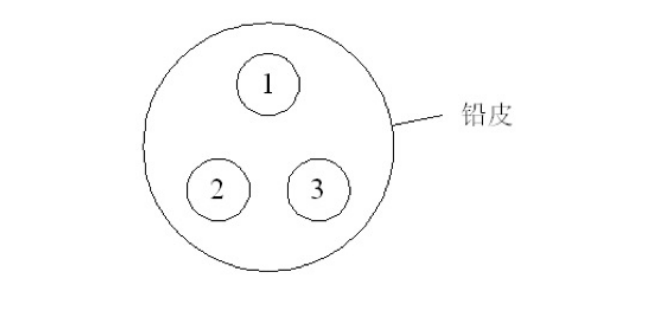
\includegraphics[width=0.4\textwidth]{4.3.png}
    \caption{三芯电缆截面图}
\end{figure}

\textbf{解答：}
设导体对地（铅皮）电容为 \(C_1\)，导体间电容为 \(C_2\)。

(1) 根据题意：
\[
\begin{cases}
3C_1 = 0.051\,\mu\text{F} \\
C_1 + 2C_2 = 0.037\,\mu\text{F}
\end{cases}
\]
解得：
\[
C_1 = 0.017\,\mu\text{F}, \quad C_2 = 0.01\,\mu\text{F}
\]
即每相导体对地电容为 \(0.017\,\mu\text{F}\)，导体间电容为 \(0.01\,\mu\text{F}\)。

(2) 每一相的工作电容为：
\[
C = C_1 + 3C_2 = 0.017 + 3 \times 0.01 = 0.047\,\mu\text{F}
\]

(3) 导体1、2之间加 \(100\,\text{V}\) 电压，导体1的电荷：
\[
Q = (C_1 + C_2)U = (0.017 + 0.01) \times 100 = 2.7\,\mu\text{C}
\]
导体2的电荷为 \(-2.7\,\mu\text{C}\)。

\vspace{1em}

%======================================================================
% 第13题（新题目6）
%======================================================================
\item 图(a)所示为镜像法分析静电场分布特性问题。两个点电荷分别位于两种介质中，两种介质的分界面为无限大平面，介电常数分别为 \(\varepsilon_1\) 和 \(\varepsilon_2\)，点电荷 \(q_1\) 与 \(q_2\) 相对于界面为镜像位置，相距为 \(2h\)。现需要用叠加定理分析介质 1 中的电位 \(\varphi_1\)：
\begin{enumerate}[label=(1)]
    \item 当考虑点电荷 \(q_1\) 单独作用时，按图(b)计算，在图(b)的括号中填入相应的介电常数，并计算 \(q_1'\)；
    \item 当考虑点电荷 \(q_2\) 单独作用时，按图(c)计算，在图(c)的括号中填入相应的介电常数，并计算 \(q_2''\)。
\end{enumerate}

\begin{figure}[htbp]
    \centering
    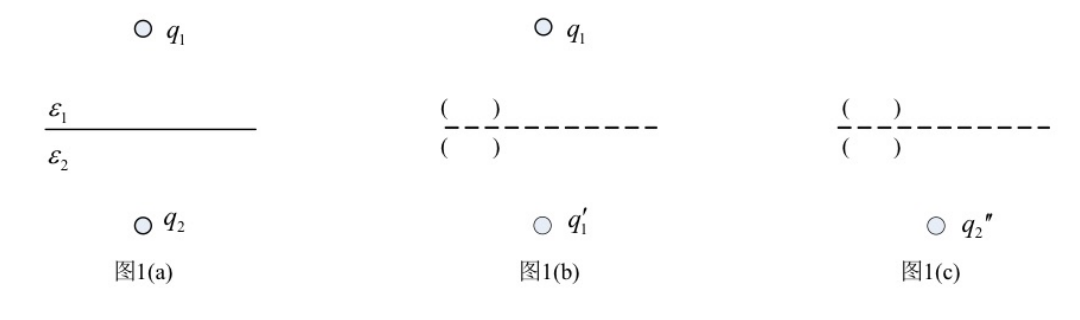
\includegraphics[width=0.4\textwidth]{4.4.png}
    \caption{镜像法分析图}
\end{figure}

\textbf{解答：}
\begin{enumerate}[label=(1)]
    \item 图(b)：介质1和介质2均为 \(\varepsilon_1\)。
    镜像电荷：
    \[
    q_1' = \frac{\varepsilon_1 - \varepsilon_2}{\varepsilon_1 + \varepsilon_2}q_1
    \]

    \item 图(c)：介质1和介质2均为 \(\varepsilon_1\)。
    镜像电荷：
    \[
    q_2'' = \frac{2\varepsilon_1}{\varepsilon_1 + \varepsilon_2}q_2
    \]
\end{enumerate}

\vspace{1em}

%======================================================================
% 第14题（新题目7）
%======================================================================
\item 试求下图所示无限长同轴电容器的单位长度电容。
\begin{figure}[htbp]
    \centering
    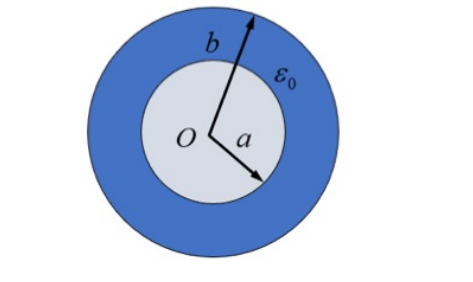
\includegraphics[width=0.3\textwidth]{4.5.png}
    \caption{同轴电容器截面图}
\end{figure}

\textbf{解答：}
内导体带单位长度电荷为 \(\tau\)，外导体带 \(-\tau\)。由高斯定理，介质内电场：
\[
\vec{E} = \frac{\tau}{2\pi\varepsilon_0 r}\vec{e}_r, \quad a<r<b
\]
内外导体间电压：
\[
U = \int_a^b \vec{E}\cdot d\vec{r} = \frac{\tau}{2\pi\varepsilon_0}\ln\frac{b}{a}
\]
单位长度电容：
\[
C = \frac{\tau}{U} = \frac{2\pi\varepsilon_0}{\ln(b/a)}
\]

\end{enumerate}